\chapter{Virologie}\label{ch:b3:virology}

Il y a quelque $10^{31}$ particules virales sur Terre, dix pour chaque
cellule, et en mer elles tuent chaque jour un cinquième de toutes les
bactéries. Un \omterm{def:b3:virology:virus}{virus} n'est pas une cellule~: il n'a ni métabolisme, ni
ribosomes, ni aucun moyen de fabriquer quoi que ce soit par lui-même.
C'est un génome --- long de deux gènes ou de deux mille --- enveloppé
d'une coque protéique, qui entre dans une cellule et détourne la
machinerie de celle-ci pour en faire des copies de lui-même. La grippe
de 1918 a tué cinquante millions de personnes~; la variole, qui a tué
trois cents millions de personnes au seul vingtième siècle, a été
éradiquée en 1980 par un \omterm{def:b3:virology:drugs}{vaccin} essayé pour la première fois en 1796~;
et un coronavirus passé à l'homme en 2019 a eu son génome séquencé en
quelques semaines, un \omterm{def:b3:virology:drugs}{vaccin} conçu dans les jours qui ont suivi, et des
médicaments contre sa protéase en deux ans. Ce chapitre traite de ce que
sont les \omterm{def:b3:virology:virus}{virus} et de la façon dont on les classe par la chimie de leur
génome, de leur multiplication, de la cinétique d'une infection à
l'intérieur d'un hôte --- qu'un couple d'équations différentielles
décrit assez bien pour avoir changé le traitement du sida --- de leur
évolution, et de la manière dont on les combat.

\section{Ce qu'est un virus}

\begin{definition}[Virus]\label{def:b3:virology:virus}
\index{virus}\index{capside}\index{enveloppe}\index{virion}\index{classification de Baltimore}
Un \emph{virus} est un parasite intracellulaire obligatoire fait d'un
génome d'acide nucléique --- ADN ou ARN, simple ou double brin,
linéaire ou circulaire, en une molécule ou plusieurs --- emballé dans
une \emph{capside} protéique et, bien souvent, enveloppé dans une
\emph{enveloppe} prise à une membrane de l'hôte et hérissée de
glycoprotéines virales. La particule infectieuse complète est le
\emph{virion}, de \qtyrange{20}{300}{nm} pour la plupart (quelques
virus géants atteignent le micromètre). Les capsides sont bâties de
nombreuses copies d'une ou de quelques protéines agencées avec une
symétrie hélicoïdale (un bâtonnet, comme chez le virus de la mosaïque
du tabac) ou icosaédrique (une coque de $60T$ sous-unités,
$T = 1, 3, 4, 7,\dots$). La \emph{classification de Baltimore} range
les virus selon la route qui mène du génome à l'ARN messager~: I, ADN
double brin (herpès, variole, adénovirus, la plupart des phages)~; II,
ADN simple brin (parvovirus)~; III, ARN double brin (rotavirus)~; IV,
ARN à brin positif, messager lui-même (polio, hépatite C, les
coronavirus)~; V, ARN à brin négatif, complémentaire du messager
(grippe, rougeole, rage, Ebola)~; VI, ARN rétrotranscrit en ADN (les
rétrovirus, le VIH)~; VII, ADN répliqué par un intermédiaire à ARN
(hépatite B). Toutes les classes sauf la première doivent apporter ou
coder une enzyme qui manque à la cellule --- une ARN polymérase
ARN-dépendante, une transcriptase inverse --- et ces enzymes sont les
cibles de la plupart des antiviraux.
\end{definition}

\begin{proof}[Faits expérimentaux]
Ivanovski (1892) et Beijerinck (1898) ont montré que la maladie de la
mosaïque du tabac se transmettait par une sève passée à travers des
filtres qui retenaient toutes les bactéries --- un \emph{contagium
vivum fluidum}, un fluide infectieux vivant. Stanley (1935) a
cristallisé l'agent, le \omterm{def:b3:virology:virus}{virus} de la mosaïque du tabac, et l'a montré
protéique avec (comme l'ont trouvé Bawden et Pirie) \qty{5}{\%} d'ARN.
Hershey et Chase (1952) ont marqué la protéine d'un bactériophage au
$^{35}$S et son ADN au $^{32}$P, l'ont laissé infecter \emph{E.~coli},
ont arraché les coques vides au mixeur, et ont trouvé le $^{32}$P à
l'intérieur des cellules et le $^{35}$S dehors~: l'ADN entre et la
protéine reste derrière, donc c'est l'ADN qui porte les instructions.
Fraenkel-Conrat (1955) a démonté le \omterm{def:b3:virology:virus}{virus} de la mosaïque du tabac en
protéine et en ARN et a réassemblé des particules infectieuses à partir
de l'ARN d'une souche et de la protéine d'une autre~; la descendance
était de la souche de l'ARN.
\end{proof}

\begin{proposition}[Économie génétique~: pourquoi les capsides sont symétriques]\label{prop:b3:virology:economy}
\index{économie génétique}
Une \omterm{def:b3:virology:virus}{capside} doit enfermer le génome qui la code. Une protéine de masse
$m$ demande environ $m/\qty{110}{Da}$ codons, soit $3m/110$
nucléotides, un tronçon d'ARN pesant environ
$3m/110\times\qty{330}{Da} = 9m$~: toute protéine est codée par un
acide nucléique neuf fois plus lourd qu'elle. Une coque faite d'une
\emph{seule} molécule de protéine enfermant un génome devrait enfermer
un génome neuf fois plus lourd qu'elle rien que pour se coder
elle-même, et une coque ne peut pas contenir neuf fois sa propre masse
d'acide nucléique à la densité biologique. L'issue, vue par Crick et
Watson (1956), est de bâtir la coque à partir de nombreuses copies
d'une petite protéine~: le \omterm{def:b3:virology:virus}{virus} de la mosaïque du tabac code une
protéine de coque de \qty{17.5}{kDa} dans \qty{480}{nt} de son génome
de \qty{6400}{nt} et en emploie $2130$ copies. Des sous-unités
identiques qui s'empilent à l'identique doivent être agencées
symétriquement, de sorte que les \omterm{def:b3:virology:virus}{capsides} virales sont des hélices ou
des icosaèdres, et la même économie leur donne la capacité de
s'auto-assembler, puisque chaque sous-unité n'a qu'à reconnaître ses
voisines.
\end{proposition}
\begin{proof}
Le rapport des masses découle de ce qu'un codon fait trois nucléotides
d'environ \qty{330}{Da} chacun et un résidu environ \qty{110}{Da}~:
$3\times 330/110 =
9$. Une \omterm{def:b3:virology:virus}{capside} faite d'une seule protéine de \qty{40}{MDa}
enfermerait \qty{360}{MDa} d'acide nucléique, une sphère d'environ
\qty{50}{nm} de rayon à la densité des acides nucléiques, alors que la
protéine elle-même ferait une coque d'environ \qty{2}{nm} d'épaisseur
et de même rayon --- géométriquement possible, mais un unique
polypeptide de $360\,000$ résidus qui se replie correctement ne l'est
pas, et une seule mutation le détruirait. Avec $n$ sous-unités
identiques le coût de codage est divisé par $n$ tandis que le volume
enfermé ne change pas.
\end{proof}

\begin{omfigure}
\begin{tikzpicture}[every node/.style={font=\scriptsize}, >=stealth]
  \node[draw, thick, rounded corners, fill=omMeth!30, minimum width=2.4cm] (mrna) at (0,0) {ARNm $\to$ protéine};
  \node[draw, thick, rounded corners, fill=omDef!20, align=center] (I) at (-5.8,3.6) {I~: ADNdb\\herpès, variole, phage T4};
  \node[draw, thick, rounded corners, fill=omDef!20, align=center] (II) at (-2.0,3.6) {II~: ADNsb\\parvovirus};
  \node[draw, thick, rounded corners, fill=omThm!20, align=center] (III) at (2.0,3.6) {III~: ARNdb\\rotavirus};
  \node[draw, thick, rounded corners, fill=omThm!20, align=center] (IV) at (5.8,3.6) {IV~: ARN(+)\\polio, hépatite C,\\coronavirus};
  \node[draw, thick, rounded corners, fill=omThm!20, align=center] (V) at (-5.6,-3.4) {V~: ARN($-$)\\grippe, rougeole,\\rage, Ebola};
  \node[draw, thick, rounded corners, fill=omProp!30, align=center] (VI) at (0,-3.4) {VI~: ARN $\to$ ADN\\rétrovirus (VIH)};
  \node[draw, thick, rounded corners, fill=omProp!30, align=center] (VII) at (5.6,-3.4) {VII~: ADN via ARN\\hépatite B};
  \node[below, font=\tiny, align=center, gray!50!black] at (-5.8,2.9) {ARN polymérase de l'hôte};
  \node[below, font=\tiny, align=center, gray!50!black] at (-2.0,3.05) {second brin fabriqué,\\puis transcription};
  \node[below, font=\tiny, align=center, gray!50!black] at (2.0,3.05) {ARN polymérase virale\\dans la particule};
  \node[below, font=\tiny, align=center, gray!50!black] at (5.8,2.75) {le génome est l'ARNm};
  \node[above, font=\tiny, align=center, gray!50!black] at (-5.6,-2.55) {une polymérase virale le copie};
  \node[above, font=\tiny, align=center, gray!50!black] at (0,-2.85) {transcriptase inverse, intégration,\\puis polymérase de l'hôte};
  \node[above, font=\tiny, align=center, gray!50!black] at (5.6,-2.85) {transcription de l'ADN};
  \foreach \c in {I,II,III,IV,V,VI,VII} \draw[->, thick] (\c) -- (mrna);
\end{tikzpicture}

{\small Les sept classes de Baltimore, rangées selon la route du génome
à l'ARN messager. Toutes sauf la première ont besoin d'une enzyme que la
cellule hôte ne fournit pas --- la cible naturelle d'un \omterm{def:b3:virology:drugs}{antiviral}.}
\end{omfigure}

\begin{omfigure}
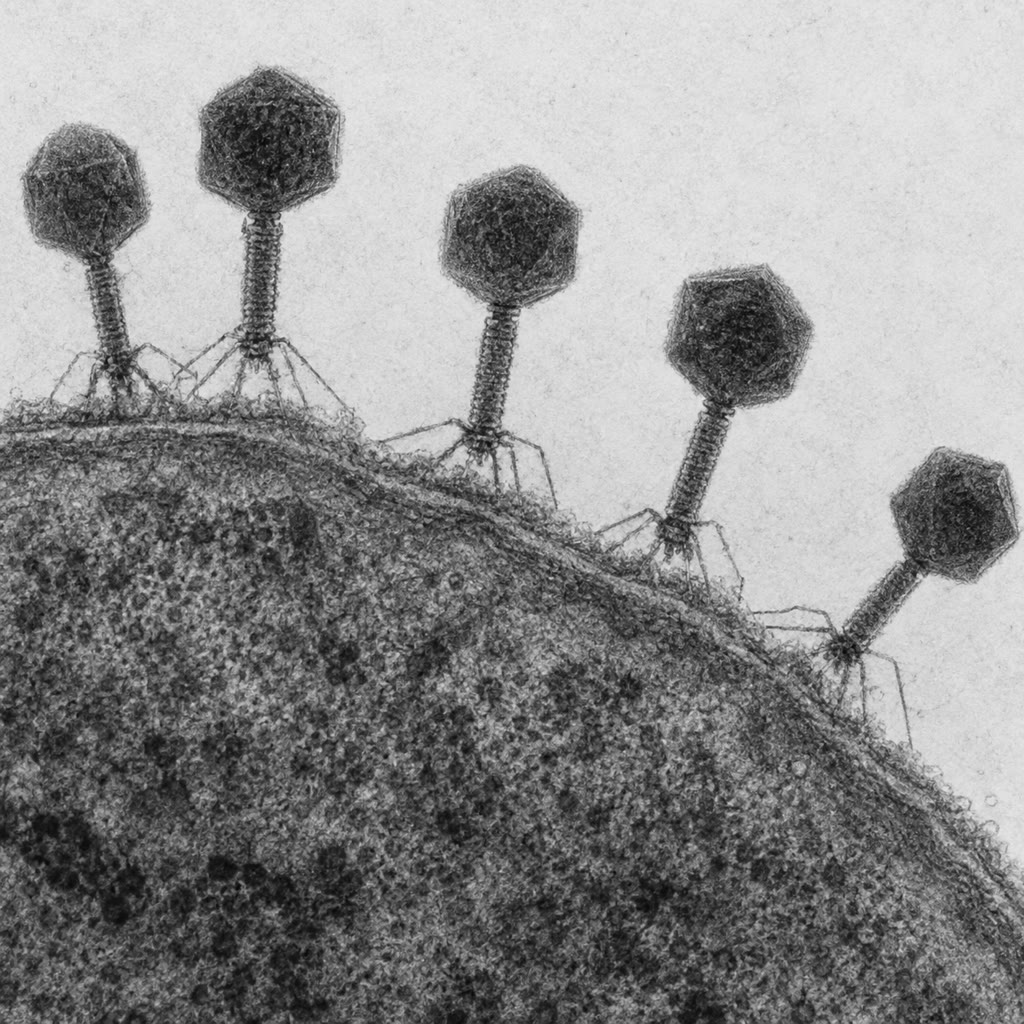
\includegraphics[width=0.36\linewidth]{images/book5/ai/b5-13-phage-tem.jpg}\hspace{0.04\linewidth}
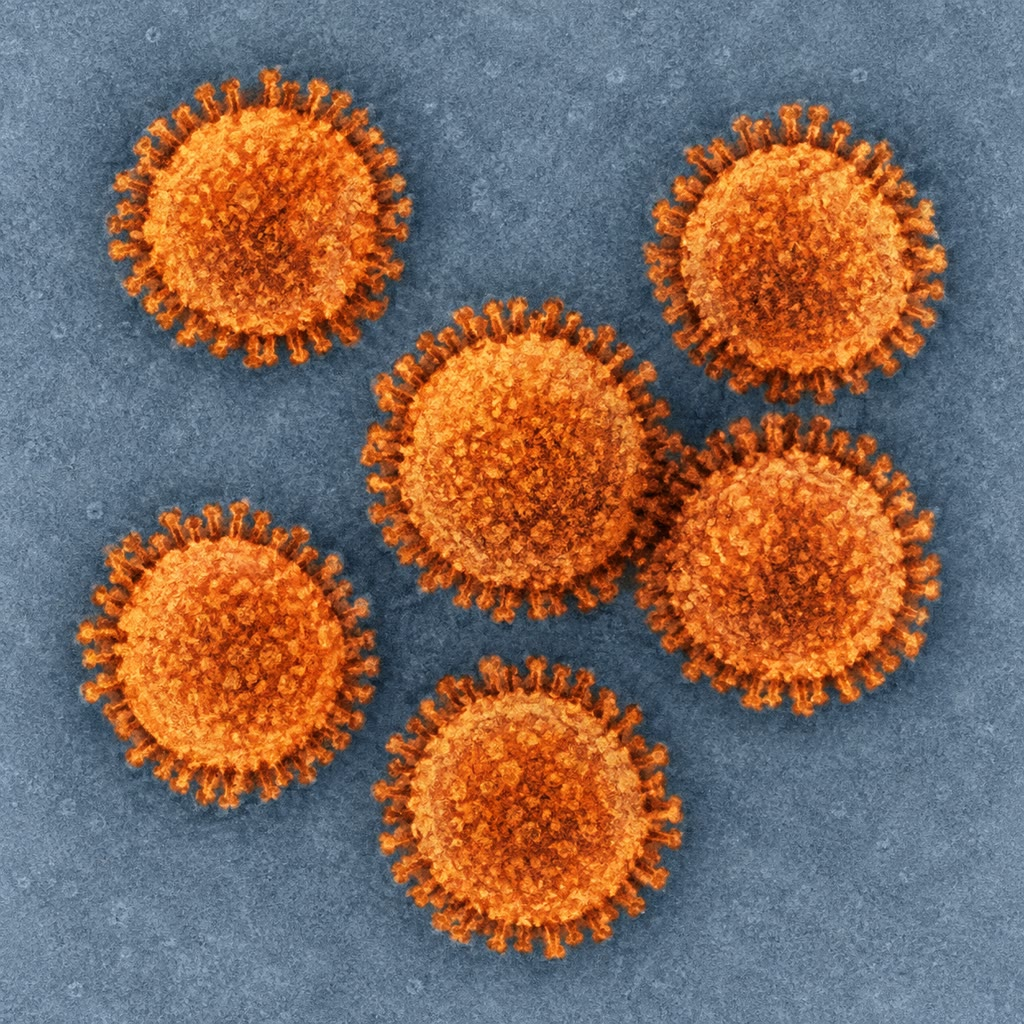
\includegraphics[width=0.36\linewidth]{images/book5/ai/b5-13-influenza-virions.jpg}

{\small À gauche~: des bactériophages accrochés par leurs fibres
caudales à une bactérie, chaque tête étant une \omterm{def:b3:virology:virus}{capside} icosaédrique
d'ADN. À droite~: des \omterm{def:b3:virology:virus}{virions} de la grippe, enveloppés, leur surface
hérissée d'hémagglutinine et de neuraminidase.}
\end{omfigure}

\section{Comment un virus se multiplie}

\begin{definition}[Le cycle de réplication]\label{def:b3:virology:cycle}
\index{cycle de réplication viral}\index{récepteur!viral}\index{lysogénie}\index{latence}
Tout \omterm{def:b3:virology:virus}{virus} passe par les mêmes étapes. L'\emph{attachement} à un
récepteur précis de l'hôte --- CD4 et un récepteur de chimiokines pour
le VIH, ACE2 pour les coronavirus du SRAS, l'acide sialique pour la
grippe, un \omterm{def:b3:bacteriology:envelope}{lipopolysaccharide} ou une porine pour un phage --- qui
décide quelles espèces et quelles cellules le \omterm{def:b3:virology:virus}{virus} peut infecter (son
\emph{tropisme}). L'\emph{entrée}~: fusion de l'\omterm{def:b3:virology:virus}{enveloppe} avec la
membrane plasmique, ou endocytose suivie d'une fusion depuis l'intérieur
de l'\omterm{def:b3:membrane-traffic:endocytosis}{endosome} acide, ou, pour un phage, injection du génome au travers
de la paroi. La \emph{décapsidation}, l'\emph{expression} des gènes
viraux par la route propre à la classe, et la \emph{réplication} du
génome, souvent dans une usine que le \omterm{def:b3:virology:virus}{virus} bâtit dans le cytoplasme ou
le noyau. L'\emph{assemblage} de nouvelles \omterm{def:b3:virology:virus}{capsides} autour de nouveaux
génomes, porté par l'auto-assemblage des sous-unités symétriques, et la
\emph{libération}~: par lyse de la cellule, ou par bourgeonnement au
travers d'une membrane, qui fournit l'\omterm{def:b3:virology:virus}{enveloppe}. Certains \omterm{def:b3:virology:virus}{virus} peuvent
au contraire insérer leur génome dans celui de l'hôte et attendre~: la
\emph{lysogénie} du phage $\lambda$, dont le répresseur le maintient
silencieux jusqu'à ce que l'hôte soit abîmé~; la \emph{latence} des
herpèsvirus dans les neurones pour toute une vie et celle du VIH sous
forme de provirus dans des lymphocytes~T au repos, d'où aucun
médicament agissant sur la réplication ne le délogera.
\end{definition}

\begin{omfigure}
\begin{tikzpicture}[every node/.style={font=\scriptsize}, >=stealth]
  % cell
  \draw[very thick, omDef, fill=omDef!6] (0,0) ellipse (5.6 and 3.2);
  \draw[thick, omDef!70, fill=omDef!20] (1.8,0) ellipse (1.6 and 1.1); \node at (1.8,0.75) {noyau};
  % virion outside
  \draw[thick, omProp, fill=omProp!30] (-7.2,1.6) circle (0.35); \foreach \a in {0,45,...,315} \draw[omProp, thick] (-7.2,1.6) ++(\a:0.35) -- ++(\a:0.15);
  \node[above] at (-7.2,2.1) {virion};
  \draw[->, thick] (-6.8,1.4) -- (-5.7,0.9); \node[below, align=center] at (-6.6,1.0) {1. attachement\\au récepteur};
  % entry
  \draw[thick, omProp] (-5.4,0.7) arc[start angle=140, end angle=40, radius=0.5];
  \node[below, align=center] at (-3.9,-0.2) {2. fusion ou endocytose~;\\3. décapsidation};
  % genome path
  \draw[omThm, very thick] (-3.4,0.2) .. controls (-2.6,0.6) .. (-1.8,0.4);
  \draw[->, thick] (-1.6,0.4) -- (-0.4,0.4);
  \node[above, align=center] at (-1.0,0.55) {4. expression des gènes,\\réplication du génome};
  \draw[omThm, very thick] (-1.0,-0.5) -- (0.4,-0.5); \draw[omThm, very thick] (-1.0,-0.75) -- (0.4,-0.75); \draw[omThm, very thick] (-1.0,-1.0) -- (0.4,-1.0);
  % assembly
  \foreach \p in {(1.2,-1.6),(1.9,-1.9),(2.6,-1.5)} { \draw[thick, omProp, fill=omProp!30] \p circle (0.25); }
  \node[below, align=center] at (1.9,-2.2) {5. assemblage des capsides\\autour des génomes};
  % budding
  \draw[thick, omProp, fill=omProp!30] (4.9,-1.7) circle (0.32); \draw[->, thick] (5.3,-1.75) -- (6.4,-2.0);
  \draw[thick, omProp, fill=omProp!30] (7.0,-2.2) circle (0.35); \foreach \a in {0,45,...,315} \draw[omProp, thick] (7.0,-2.2) ++(\a:0.35) -- ++(\a:0.15);
  \node[below, align=center] at (6.4,-2.6) {6. bourgeonnement\\(enveloppe)\\ou lyse de la cellule};
  % latency
  \draw[->, thick, dashed, omMeth!70!black] (-0.2,0.2) -- (0.9,0.2); \node[below, omMeth!70!black, align=center, font=\tiny] at (2.0,-0.05) {rétrovirus~: intégration\\en provirus~; latence};
\end{tikzpicture}

{\small Le cycle de réplication d'un \omterm{def:b3:virology:virus}{virus} enveloppé~: attachement à un
récepteur, entrée et décapsidation, expression et réplication dans la
machinerie de l'hôte, assemblage, et libération par bourgeonnement ---
ou, pour un rétrovirus, intégration dans le génome de l'hôte et
silence.}
\end{omfigure}

\begin{method}[Compter les particules infectieuses~: le test des plages]\label{met:b3:virology:plaque}
\index{test des plages}\index{titre}
Pour mesurer un lot de \omterm{def:b3:virology:virus}{virus}~: (1) le diluer par paliers de dix~;
(2) mélanger chaque dilution à un excès de cellules hôtes --- des
bactéries en gélose molle pour un phage, une monocouche de cellules en
culture pour un \omterm{def:b3:virology:virus}{virus} animal~; (3) incuber~: chaque particule
infectieuse infecte une cellule, la descendance infecte les voisines,
et au bout d'un jour ou deux un trou clair, une \emph{plage}, marque
l'endroit~; (4) compter les plages sur une boîte qui en porte
\numrange{30}{300} et multiplier par la dilution~: c'est le \emph{titre}
en unités formant plage (UFP) par millilitre. Puisque chaque plage est
le clone d'une particule, en prélever une donne un isolat pur. Le
rapport des particules physiques (comptées au microscope électronique
ou par PCR) aux unités formant plage dépasse largement un --- de dix à
mille pour bien des \omterm{def:b3:virology:virus}{virus} animaux --- puisque la plupart des particules
sont défectueuses ou n'arrivent pas à infecter.
\end{method}

\begin{omfigure}
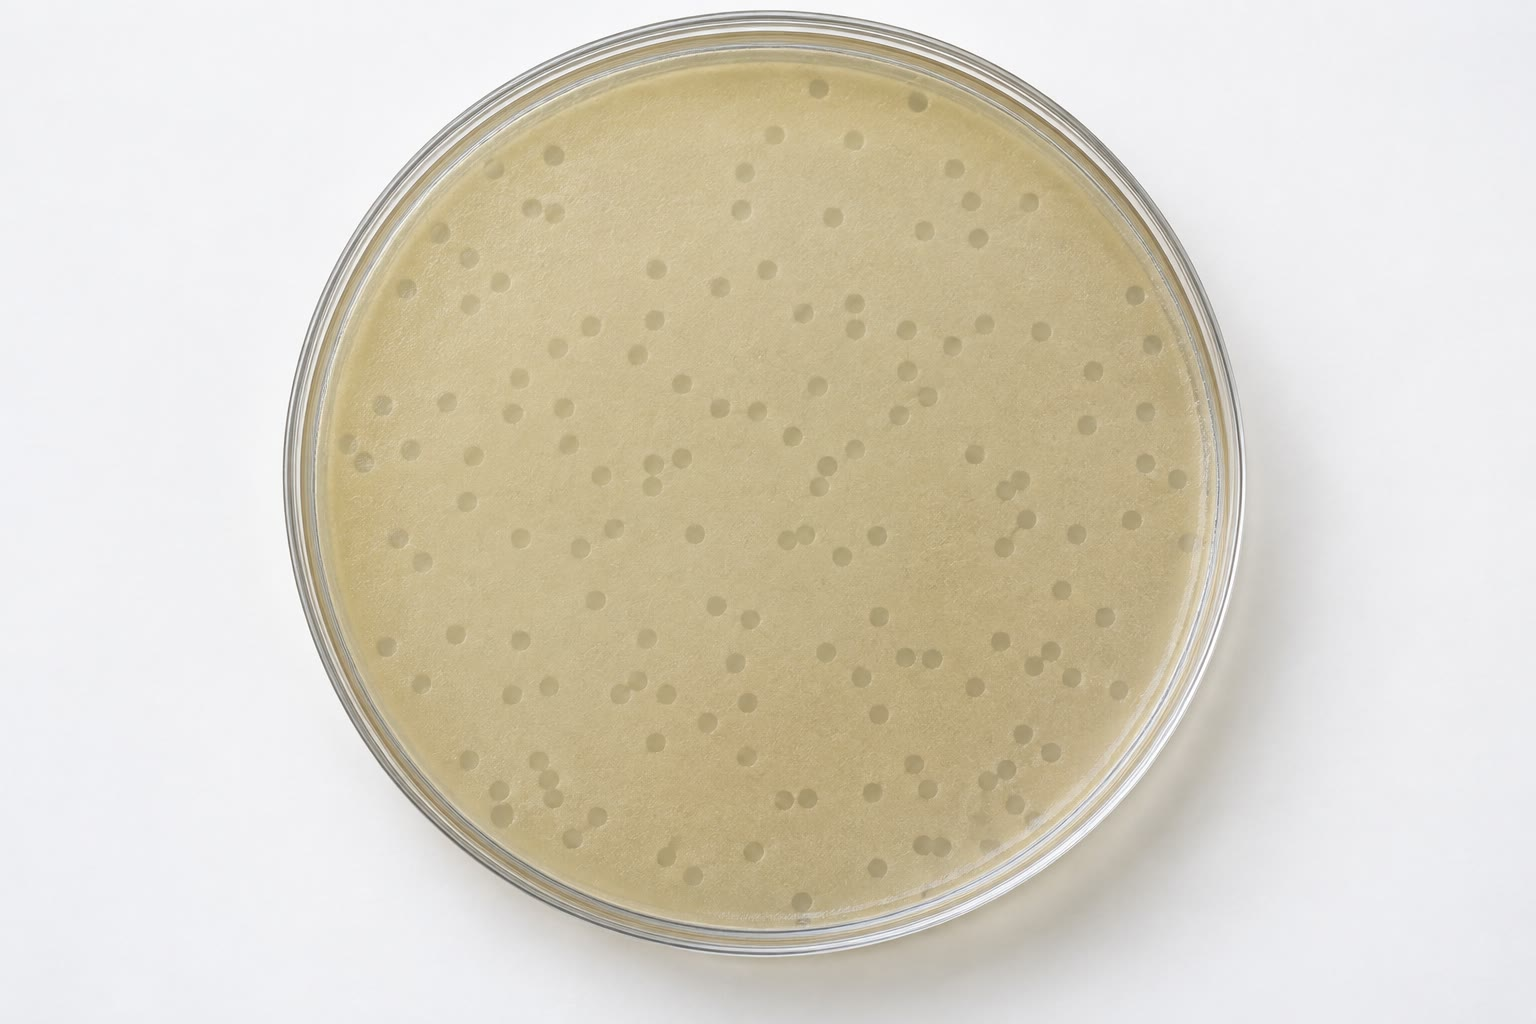
\includegraphics[width=0.46\linewidth]{images/book5/ai/b5-13-plaque-assay.jpg}\hspace{0.04\linewidth}
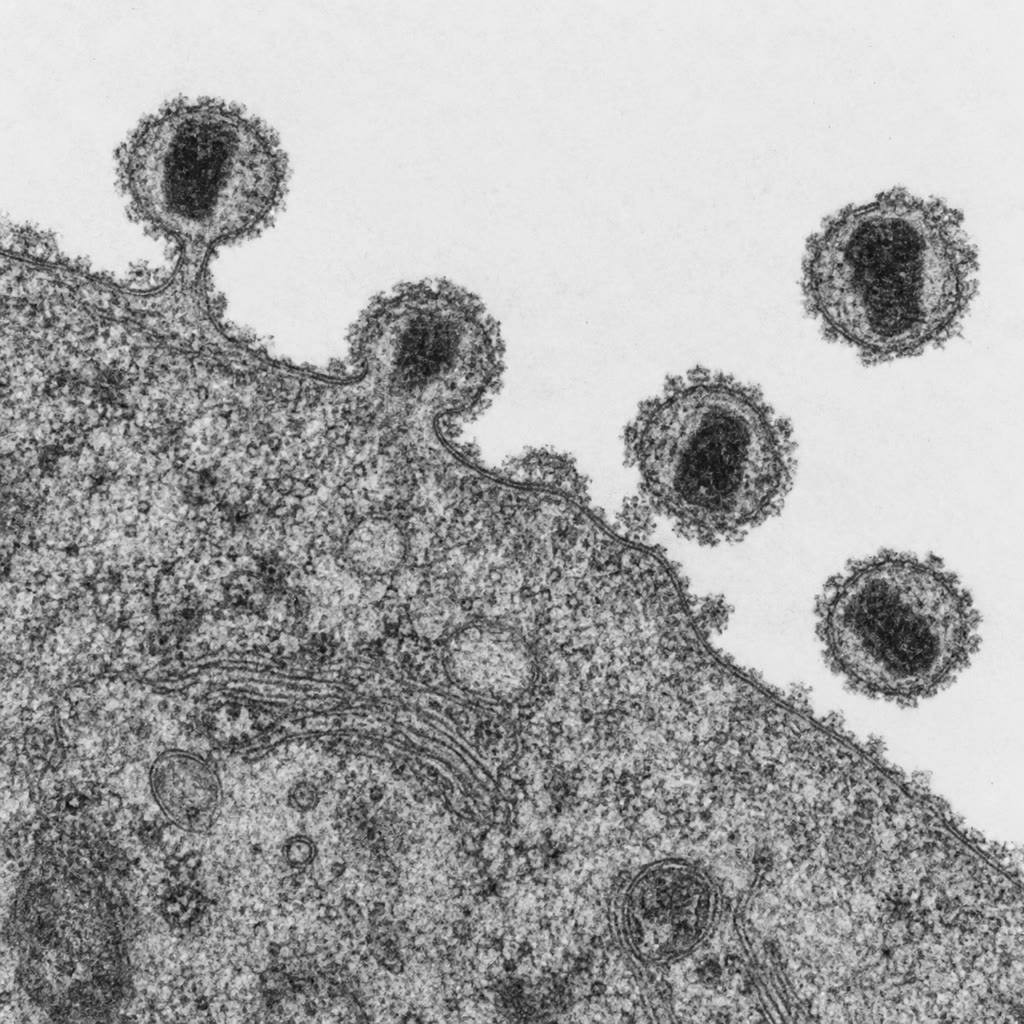
\includegraphics[width=0.36\linewidth]{images/book5/ai/b5-13-hiv-budding.jpg}

{\small À gauche~: des plages dans un tapis bactérien, chacune une zone
claire où la descendance d'un phage a lysé les cellules autour de lui. À
droite~: des particules de VIH bourgeonnant d'un lymphocyte~T, qui
prennent leur \omterm{def:b3:virology:virus}{enveloppe} à la membrane de la cellule.}
\end{omfigure}

\begin{theorem}[Dynamique de l'infection chez un hôte]\label{thm:b3:virology:dynamics}
\index{taux de reproduction de base!intra-hôte}\index{charge virale}\index{dynamique virale}
Soit $T$ la densité de cellules cibles sensibles, $I$ celle de cellules
infectées et $V$ celle de \omterm{def:b3:virology:virus}{virions} libres. Les \omterm{def:b3:virology:virus}{virions} infectent les
cibles à la vitesse $\beta TV$, les cellules infectées produisent
chacune des \omterm{def:b3:virology:virus}{virions} à la vitesse $p$ et meurent à la vitesse $\delta$,
et les \omterm{def:b3:virology:virus}{virions} libres sont éliminés à la vitesse $c$~:
\[
\frac{\mathrm{d}I}{\mathrm{d}t} = \beta TV - \delta I, \qquad
\frac{\mathrm{d}V}{\mathrm{d}t} = pI - cV .
\]
À $T$ maintenu constant, l'infection croît si le \emph{taux de
reproduction de base} $R_{0} = \beta Tp/(c\delta)$ dépasse $1$, et à
l'état stationnaire $V^{*} = p I^{*}/c$, la production équilibrant
l'élimination. Si un médicament arrête toute nouvelle infection en
$t = 0$ ($\beta \to 0$), les \omterm{def:b3:virology:virus}{virions} décroissent d'abord à la vitesse
d'élimination $c$, puis, une fois le \omterm{def:b3:virology:virus}{virus} libre retombé au niveau que
les cellules infectées restantes entretiennent, à la vitesse de mort
$\delta$ de ces cellules~:
\[
V(t) \approx V_{0}\,\frac{c\,e^{-\delta t} - \delta\,e^{-ct}}{c - \delta}
\;\longrightarrow\; V_{0}\,\frac{c}{c-\delta}\,e^{-\delta t}
\quad (t \gg 1/c).
\]
Les deux pentes de la \omterm{thm:b3:virology:dynamics}{charge virale} après traitement mesurent $c$ et
$\delta$, et $pI^{*} = cV^{*}$ donne la production quotidienne de
\omterm{def:b3:virology:virus}{virions} avant traitement.
\end{theorem}
\begin{proof}
Une cellule infectée vit en moyenne $1/\delta$ et fabrique $p/\delta$
\omterm{def:b3:virology:virus}{virions}~; chaque \omterm{def:b3:virology:virus}{virion} vit $1/c$ et infecte $\beta T/c$ cellules
pendant ce temps~; le produit est le nombre de cellules infectées
qu'une cellule infectée engendre, $R_{0}$. À l'état stationnaire
$\mathrm{d}V/\mathrm{d}t = 0$ donne $V^{*} = pI^{*}/c$. Après
traitement $\mathrm{d}I/\mathrm{d}t =
-\delta I$, donc $I = I_{0}e^{-\delta t}$, et $\mathrm{d}V/\mathrm{d}t =
pI_{0}e^{-\delta t} - cV$ est une équation linéaire dont la solution
avec $V(0) = V_{0} = pI_{0}/c$ est l'expression donnée (vérification~:
en $t = 0$ elle vaut $V_{0}$, et elle satisfait l'équation terme à
terme). Pour $t
\gg 1/c$ le terme $e^{-ct}$ a disparu et $V$ suit les cellules infectées
avec la pente $-\delta$~; pour $t \ll 1/\delta$ et $c \gg \delta$ la
pente initiale vaut $-c$.
\end{proof}

\begin{example}[Le VIH avant et après les équations]\label{ex:b3:virology:hiv}
Jusqu'en 1995, les années de \omterm{def:b3:virology:cycle}{latence} clinique de l'infection par le VIH
--- une \omterm{thm:b3:virology:dynamics}{charge virale} stable de $10^{4}$--$10^{6}$ copies par
millilitre et une lente chute des lymphocytes~T --- se lisaient comme un
\omterm{def:b3:virology:virus}{virus} au repos. Ho, Perelson et leurs collègues ont donné à des
patients un \omterm{def:b3:virology:drugs}{inhibiteur de protéase} et ont ajusté la décroissance de la
\omterm{thm:b3:virology:dynamics}{charge virale} au théorème~: la phase rapide a donné
$c \approx \qty{3}{d^{-1}}$ (une demi-vie du \omterm{def:b3:virology:virus}{virion} d'environ six
heures), la phase lente $\delta \approx
\qty{0.5}{d^{-1}}$ (une cellule infectée vit environ un jour et demi).
Une charge stable de $10^{5}$ par millilitre dans \qty{15}{L} de
liquides corporels, éliminée à $c$, exige donc la production d'environ
$10^{10}$ \omterm{def:b3:virology:virus}{virions} par jour, chaque jour, pendant des années~: la
période «~latente~» est un état stationnaire furieux d'infection et de
mort, le stock de lymphocytes~T étant remplacé chaque jour jusqu'à ce
qu'il cède. L'arithmétique des mutations de la section suivante en
découle aussitôt, et avec elle la raison pour laquelle les médicaments
seuls ont échoué et trois ensemble non.
\end{example}

\begin{omfigure}
\begin{tikzpicture}
\begin{axis}[
  width=0.7\linewidth, height=5.8cm,
  axis x line=bottom, axis y line=left,
  xmin=0, xmax=14, ymin=10, ymax=2e5, ymode=log,
  xlabel={jours après le début du traitement}, ylabel={virions par mL},
  xlabel style={font=\small, at={(axis description cs:0.5,-0.12)}, anchor=north}, ylabel style={font=\small},
  tick label style={font=\small}, xtick={0,2,4,6,8,10,12,14},
  clip=false,
]
\addplot[very thick, omDef, domain=0:14, samples=100] {1e5*(3*exp(-0.5*x) - 0.5*exp(-3*x))/2.5};
\addplot[dashed, omThm, domain=0:1.6, samples=2] {1e5*exp(-3*x)};
\addplot[dashed, omMeth!70!black, domain=1.5:14, samples=2] {1e5*1.2*exp(-0.5*x)};
\node[font=\scriptsize, omThm, anchor=west] at (axis cs:1.8,600) {virions libres éliminés~: pente $-c$, demi-vie \qty{6}{h}};
\node[font=\scriptsize, omMeth!70!black, anchor=south west] at (axis cs:5.5,1.5e4) {cellules infectées qui meurent~: pente $-\delta$, demi-vie \qty{1.4}{d}};
\end{axis}
\end{tikzpicture}

{\small \omterm{thm:b3:virology:dynamics}{Charge virale} après qu'un médicament a arrêté les nouvelles
infections, d'après le théorème avec $c = \qty{3}{d^{-1}}$ et
$\delta = \qty{0.5}{d^{-1}}$~: une chute rapide pendant que les \omterm{def:b3:virology:virus}{virions}
libres sont éliminés, puis une chute plus lente au rythme de la mort
des cellules déjà infectées.}
\end{omfigure}

\section{Comment les virus évoluent}

\begin{definition}[Mutation, quasi-espèce, glissement et cassure]\label{def:b3:virology:evolution}
\index{quasi-espèce}\index{glissement antigénique}\index{cassure antigénique}\index{réassortiment}
Les polymérases ARN-dépendantes et les transcriptases inverses n'ont
pas de relecture, et les \omterm{def:b3:virology:virus}{virus} à ARN mutent à $10^{-4}$ à $10^{-6}$ par
nucléotide et par réplication --- mille à un million de fois le taux de
leurs hôtes --- de sorte que la population d'un \omterm{def:b3:virology:virus}{virus} à ARN est un nuage
de génomes apparentés, une \emph{quasi-espèce}, où tout mutant ponctuel
est présent à chaque instant si la population est grande. La sélection
par les anticorps entraîne le \emph{glissement antigénique}~: les
protéines de surface de la grippe accumulent des substitutions année
après année, et l'immunité de l'an dernier protège un peu moins à
chaque saison. La \emph{cassure antigénique} est un saut~: un génome
segmenté (la grippe a huit segments d'ARN) peut être \emph{réassorti}
quand deux souches infectent une même cellule, et un segment codant une
hémagglutinine d'un \omterm{def:b3:virology:virus}{virus} d'oiseau ou de porc, contre laquelle aucun
humain n'est immunisé, produit une pandémie --- 1918, 1957, 1968, 2009.
La recombinaison à l'intérieur d'un génome fait de même pour les \omterm{def:b3:virology:virus}{virus}
non segmentés, et les coronavirus recombinent volontiers. La plupart
des \omterm{def:b3:virology:virus}{virus} humains nouveaux sont des \emph{zoonoses}, venues d'un
réservoir animal --- les chauves-souris pour les coronavirus, Ebola et
la rage~; les oiseaux et les porcs pour la grippe~; les primates pour
le VIH --- et le passage n'est en général qu'affaire de quelques
mutations dans une protéine de fixation au récepteur.
\end{definition}

\begin{proposition}[Le seuil d'erreur]\label{prop:b3:virology:error-threshold}
\index{seuil d'erreur}\index{relecture!virale}
Un génome de $L$ nucléotides copié avec un taux d'erreur $u$ par
nucléotide est copié sans aucune erreur avec la probabilité
$(1-u)^{L} \approx e^{-uL}$. Pour que la séquence la mieux adaptée
persiste dans la population contre le flot de ses mutants, la fraction
de copies sans erreur doit dépasser à peu près l'inverse de son
avantage sélectif $\sigma$~: $e^{-uL} \gtrsim
1/\sigma$, c'est-à-dire $uL \lesssim \ln\sigma$, un nombre d'ordre un.
Le produit du taux de mutation par la longueur du génome est donc
borné~: un \omterm{def:b3:virology:virus}{virus} à ARN de $u = 10^{-4}$ ne peut pas avoir un génome
beaucoup plus long que $10^{4}$ nucléotides, ce qui est à peu près ce
qu'ont les \omterm{def:b3:virology:virus}{virus} à ARN, et les coronavirus, avec \qty{30}{kb} les plus
longs génomes à ARN connus, n'y parviennent qu'en codant une
exonucléase de relecture qui divise $u$ par dix. Le seuil est aussi une
arme~: des médicaments qui élèvent le taux d'erreur de la polymérase
(ribavirine, molnupiravir) poussent un \omterm{def:b3:virology:virus}{virus} au-delà, dans la
\emph{catastrophe d'erreur}, et la \omterm{def:b3:virology:evolution}{quasi-espèce} s'effondre.
\end{proposition}
\begin{proof}
Des erreurs indépendantes à chacun des $L$ sites donnent la probabilité
de copie sans erreur $(1-u)^{L}$, et $\ln(1-u) \approx -u$ pour $u$
petit. Le bilan de population est l'argument classique des
\omterm{def:b3:virology:evolution}{quasi-espèces} (Eigen, 1971)~: la séquence maîtresse est reconstituée à
la vitesse $\sigma e^{-uL}$ par rapport au mutant moyen et perdue par
mutation autrement~; elle ne se maintient que si la première dépasse
$1$, d'où la borne.
\end{proof}

\begin{omfigure}
\begin{tikzpicture}[every node/.style={font=\scriptsize}, >=stealth]
  % drift
  \begin{scope}
    \foreach \i in {0,1,2,3} { \draw[thick, omProp, fill=omProp!30] (\i*1.3,0) circle (0.35); \foreach \a in {0,60,...,300} \draw[omProp, thick] (\i*1.3,0) ++(\a:0.35) -- ++(\a:0.14); }
    \foreach \i/\n in {1/1,2/2,3/3} { \foreach \k in {1,...,\n} \fill[omThm] (\i*1.3,0) ++({60*\k+20}:0.5) circle (0.06); }
    \foreach \i in {0,1,2} \draw[->, thick] (\i*1.3+0.5,0) -- (\i*1.3+0.8,0);
    \node[below, align=center] at (1.95,-0.6) {glissement antigénique~: des mutations\\ponctuelles s'accumulent dans les protéines\\de surface, saison après saison};
  \end{scope}
  % shift
  \begin{scope}[xshift=7.0cm]
    \draw[thick, omProp, fill=omProp!30] (0,0.5) circle (0.4); \foreach \y in {-0.2,-0.1,0,0.1,0.2} \draw[omProp!80!black] (-0.25,0.5+\y) -- (0.25,0.5+\y);
    \draw[thick, omMeth!70!black, fill=omMeth!30] (0,-0.7) circle (0.4); \foreach \y in {-0.2,-0.1,0,0.1,0.2} \draw[omMeth!70!black] (-0.25,-0.7+\y) -- (0.25,-0.7+\y);
    \node[left, align=right] at (-0.5,0.5) {souche humaine,\\8 segments}; \node[left, align=right] at (-0.5,-0.7) {souche aviaire,\\8 segments};
    \draw[->, thick] (0.5,0.4) -- (1.5,0.0); \draw[->, thick] (0.5,-0.6) -- (1.5,-0.2);
    \draw[thick, omDef, fill=omDef!10] (2.4,-0.1) ellipse (0.9 and 0.7); \node[below] at (2.4,-0.85) {une cellule (d'un porc)};
    \draw[->, thick] (3.4,-0.1) -- (4.3,-0.1);
    \draw[thick, omProp, fill=omProp!30] (4.9,-0.1) circle (0.4); \foreach \y in {-0.2,-0.1,0.1,0.2} \draw[omProp!80!black] (4.65,-0.1+\y) -- (5.15,-0.1+\y); \draw[omMeth!70!black, very thick] (4.65,-0.1) -- (5.15,-0.1);
    \node[right, align=left] at (5.4,-0.1) {réassortant~:\\hémagglutinine\\aviaire dans un\\virus humain};
    \node[below, align=center] at (2.4,-1.5) {cassure antigénique~: segments entiers échangés~;\\personne n'est immunisé --- pandémie};
  \end{scope}
\end{tikzpicture}

{\small Deux façons pour un \omterm{def:b3:virology:virus}{virus} de la grippe d'échapper à l'immunité.
Le glissement~: les mutations des spicules s'accumulent peu à peu. La
cassure~: deux souches dans une même cellule échangent des segments
entiers de génome, et une protéine de spicule nouvelle pour l'homme
apparaît d'un coup.}
\end{omfigure}

\begin{example}[Pourquoi le VIH a exigé trois médicaments]\label{ex:b3:virology:three-drugs}
La transcriptase inverse du VIH se trompe environ une fois sur $10^{5}$
nucléotides, de sorte que chaque génome de \qty{9700}{nt} copié porte
environ $0.1$ mutation, et que $10^{10}$ génomes neufs par jour en
portent $10^{9}$ à eux tous~: chacune des
$3\times 9700 \approx \num{30000}$ mutations ponctuelles possibles
apparaît de nombreuses fois chaque jour, avant même qu'aucun médicament
soit donné. Un médicament qu'une seule mutation met en échec --- comme
une seule mutation met en échec la plupart des inhibiteurs de la
transcriptase inverse et de la protéase --- est donc défait en quelques
semaines, ce qui est arrivé à l'AZT en 1987. Deux mutations
indépendantes apparaissent ensemble à $10^{-10}$ par génome, soit
environ une fois par jour~; trois à $10^{-15}$, une fois en mille jours
--- et un patient sous trois médicaments dont la charge a chuté d'un
facteur mille produit $10^{7}$ génomes par jour, de sorte que le triple
mutant n'apparaît jamais. Cela, et la démonstration par le théorème que
le \omterm{def:b3:virology:virus}{virus} se répliquait à plein régime, ont fait de la trithérapie, dès
1996, le traitement qui a fait du sida une maladie chronique.
\end{example}

\section{Hôtes, défenses et médicaments}

\begin{proposition}[Pathogénie et défense]\label{prop:b3:virology:pathogenesis}
\index{effet cytopathique}\index{interféron}\index{restriction!des phages}
Un \omterm{def:b3:virology:virus}{virus} nuit en lysant des cellules (la polio détruit les
motoneurones, le VIH tue des lymphocytes~T), en faisant produire aux
cellules des produits toxiques, en les transformant
(\cref{ch:b3:cancer-biology}), et souvent surtout par la réponse de
l'hôte lui-même~: la fièvre, les lésions tissulaires et, au pire,
l'orage cytokinique de la réaction immunitaire à la grippe ou aux
coronavirus du SRAS. L'hôte répond par des défenses innées qui
reconnaissent les signatures d'une réplication virale --- ARN double
brin, ARN sans coiffe, ADN dans le cytosol --- et par
l'\emph{interféron}, qui met chaque cellule voisine en état \omterm{def:b3:virology:drugs}{antiviral}
(\cref{ch:b3:innate-immunity})~; par des cellules tueuses naturelles
qui détruisent les cellules ayant caché leur CMH~; par des anticorps
qui neutralisent les \omterm{def:b3:virology:virus}{virions} et des lymphocytes~T cytotoxiques qui
tuent les cellules infectées avant qu'elles ne libèrent leur
descendance (\cref{ch:b3:adaptive-immunity})~; et, chez les bactéries,
par des \omterm{def:b3:genetic-engineering:tools}{enzymes de restriction} qui coupent l'ADN étranger et par la
mémoire \omterm{def:b3:genetic-engineering:crispr}{CRISPR} du \cref{ch:b3:genetic-engineering}. Les \omterm{def:b3:virology:virus}{virus}
répliquent~: presque tout grand \omterm{def:b3:virology:virus}{virus} code des protéines qui bloquent
l'interféron, cachent le CMH, imitent des cytokines ou inhibent
l'\omterm{def:b3:cell-cycle-apoptosis:apoptosis}{apoptose}, et la course aux armements est inscrite dans les deux
génomes.
\end{proposition}

\begin{definition}[Antiviraux et vaccins]\label{def:b3:virology:drugs}
\index{antiviral}\index{analogue nucléosidique}\index{inhibiteur de protéase}\index{vaccin}\index{vaccin à ARN messager}
Les antiviraux s'attaquent aux enzymes virales ou aux étapes qu'une
cellule hôte n'accomplit pas. Les \emph{analogues nucléosidiques} sont
des terminateurs de chaîne~: l'aciclovir n'est phosphorylé que par la
thymidine kinase de l'herpèsvirus et bloque ensuite l'ADN polymérase
virale, de sorte qu'il n'agit que dans les cellules infectées~; l'AZT,
le ténofovir et la lamivudine arrêtent la transcriptase inverse~; le
remdésivir et le molnupiravir agissent sur la polymérase des
coronavirus, le second par mutagenèse. Les \emph{inhibiteurs de
protéase} bloquent le clivage des polyprotéines virales (VIH,
hépatite C, le nirmatrelvir contre le SARS-CoV-2). Les inhibiteurs
d'intégrase empêchent la formation du provirus du VIH~; les inhibiteurs
de neuraminidase empêchent les \omterm{def:b3:virology:virus}{virions} de la grippe de se détacher de
la cellule dont ils bourgeonnent~; les inhibiteurs d'entrée bloquent un
récepteur. Le \omterm{def:b3:virology:virus}{virus} de l'hépatite C se guérit aujourd'hui en douze
semaines par des associations de médicaments à action directe, première
infection virale chronique jamais guérie par une chimiothérapie. Les
\emph{vaccins} présentent les antigènes du \omterm{def:b3:virology:virus}{virus} sans sa maladie~: un
\omterm{def:b3:virology:virus}{virus} vivant atténué (rougeole, polio par voie orale, fièvre jaune), un
\omterm{def:b3:virology:virus}{virus} inactivé (polio injectable, grippe), une sous-unité (l'antigène
de surface de l'hépatite B fabriqué dans la levure, la protéine de
\omterm{def:b3:virology:virus}{capside} du papillomavirus), un vecteur viral inoffensif porteur d'un
gène de la cible, ou, depuis 2020, un \emph{ARN messager} codant
l'antigène, livré dans des nanoparticules lipidiques, que les cellules
mêmes du vacciné traduisent. L'immunologie qui explique pourquoi ils
marchent, et combien de personnes il faut vacciner pour protéger les
autres, fait l'objet du \cref{ch:b3:adaptive-immunity}.
\end{definition}

\begin{remark}[Les virus dans l'économie du vivant]\label{rem:b3:virology:economy}
Les \omterm{def:b3:virology:virus}{virus} qui nuisent à l'homme sont une erreur d'arrondi dans la
population virale du monde, qui infecte surtout des bactéries et des
archées. Les phages tuent chaque jour un cinquième à un tiers des
bactéries de l'océan et en rendent le contenu au stock dissous --- le
\emph{court-circuit viral} du cycle du carbone du volume de deuxième
année. Ils déplacent des gènes entre bactéries
(\cref{ch:b3:bacteriology}), et leurs toxines sont celles de la
diphtérie, du choléra et des pires \emph{E.~coli}. Huit pour cent du
génome humain sont les restes de rétrovirus anciens
(\cref{ch:b3:genomics}), et l'un de leurs gènes d'\omterm{def:b3:virology:virus}{enveloppe} fusionne
aujourd'hui les cellules du placenta. Les \omterm{def:b3:virology:virus}{virus} sont le plus grand
réservoir de nouveauté génétique de la planète, et la frontière de ce
qui compte comme vivant passe par eux.
\end{remark}

\section{Exercices}

\begin{exercise}[$\star$]\label{exo:b3:virology:1}
Placer la polio, la grippe, le VIH, l'herpès simplex, l'hépatite B et
le rotavirus dans leurs classes de Baltimore et dire quelle enzyme
chacun doit apporter ou fabriquer et qui manque à la cellule.
\end{exercise}

\begin{exercise}[$\star$]\label{exo:b3:virology:2}
Qu'a montré l'expérience de Hershey et Chase, et qu'aurait-on trouvé si
la protéine avait porté les instructions~?
\end{exercise}

\begin{exercise}[$\star$]\label{exo:b3:virology:3}
Un lot de phages dilué au $10^{-7}$ donne $84$ plages à partir de
\qty{0.1}{mL}. Quel est le titre~? Pourquoi le microscope électronique
peut-il compter dix fois plus de particules~?
\end{exercise}

\begin{exercise}[$\star$]\label{exo:b3:virology:4}
Énumérer les six étapes d'un cycle de réplication et, pour chacune,
nommer un \omterm{def:b3:virology:drugs}{antiviral} ou une défense de l'hôte qui y agit.
\end{exercise}

\begin{exercise}[$\star\star$]\label{exo:b3:virology:5}
À l'aide de la \cref{prop:b3:virology:economy}, calculer l'acide
nucléique nécessaire pour coder la \omterm{def:b3:virology:virus}{capside} d'un \omterm{def:b3:virology:virus}{virus} fait de $180$
copies d'une protéine de \qty{30}{kDa}, et comparer au génome de
\qty{4.5}{kb} qu'un tel \omterm{def:b3:virology:virus}{virus} pourrait avoir. Quelle fraction du génome
le gène de la \omterm{def:b3:virology:virus}{capside} représente-t-il~?
\end{exercise}

\begin{exercise}[$\star\star$]\label{exo:b3:virology:6}
Avec $c = \qty{3}{d^{-1}}$, $\delta = \qty{0.5}{d^{-1}}$ et $V_{0} =
10^{5}$ par mL, calculer $V$ d'après le théorème en $t = 0.5$, $2$ et
$10$ jours. Au bout de combien de temps la charge tombe-t-elle sous
$50$ par mL, la limite de détection~?
\end{exercise}

\begin{exercise}[$\star\star$]\label{exo:b3:virology:7}
Un \omterm{def:b3:virology:virus}{virus} à ARN a $u = 3\times 10^{-5}$ et $L = \qty{12}{kb}$. Quelle
fraction de sa descendance ne porte aucune mutation~? Qu'advient-il de
cette fraction si un médicament mutagène triple $u$~? Expliquer
pourquoi les coronavirus ont eu besoin d'une enzyme de relecture.
\end{exercise}

\begin{exercise}[$\star\star$]\label{exo:b3:virology:8}
Expliquer le glissement et la \omterm{def:b3:virology:evolution}{cassure antigéniques} de la grippe, et
pourquoi une souche pandémique a jusqu'ici toujours porté une
hémagglutinine nouvelle.
\end{exercise}

\begin{exercise}[$\star\star$]\label{exo:b3:virology:9}
L'aciclovir est un analogue de la guanosine qui doit être phosphorylé
pour agir. Expliquer pourquoi il nuit aux cellules infectées par
l'herpès et non aux autres, et prévoir les mutations de résistance.
\end{exercise}

\begin{exercise}[$\star\star\star$]\label{exo:b3:virology:10}
Établir $R_{0} = \beta Tp/(c\delta)$ à partir des deux équations du
théorème, en cherchant la condition pour qu'une petite infection ($I$
et $V$ voisins de zéro, $T$ constant) croisse, et interpréter chaque
facteur.
\end{exercise}

\begin{exercise}[$\star\star\star$]\label{exo:b3:virology:11}
Un patient sous traitement efficace abrite encore $10^{6}$ lymphocytes~T
au repos infectés de façon latente, dont le provirus est silencieux,
avec une demi-vie de $44$ mois. Combien de temps le traitement
devrait-il durer pour que le réservoir tombe sous une cellule~?
Pourquoi cela rend-il le VIH incurable par des médicaments qui bloquent
la réplication, et qu'exigerait une guérison~?
\end{exercise}

\begin{exercise}[$\star\star\star$]\label{exo:b3:virology:12}
Reprendre l'argument de l'\cref{ex:b3:virology:three-drugs} avec vos
propres nombres pour un \omterm{def:b3:virology:virus}{virus} de \qty{30}{kb} de $u = 10^{-6}$
produisant $10^{9}$ génomes par jour. Combien de médicaments
associeriez-vous, et pourquoi des médicaments visant deux sites d'une
même enzyme pourraient-ils ne pas compter pour deux~?
\end{exercise}

\section{Problème~: un virus chez un patient}

\begin{problem}[{Problème du week-end --- une infection par le VIH
comptée virion par virion, sa dynamique ajustée sur une courbe de
traitement, ses mutations dénombrées face aux médicaments et son
réservoir chronométré, pour finir sur la production quotidienne de
virions, le jour où la charge devient indétectable et la probabilité
qu'un triple mutant existe}]
\label{pb:b3:virology:1}
Données~: \omterm{thm:b3:virology:dynamics}{charge virale} $V^{*} = 2\times 10^{5}$ par mL dans
\qty{15}{L} de liquides corporels~; $c = \qty{3}{d^{-1}}$,
$\delta = \qty{0.5}{d^{-1}}$~; chaque cellule infectée fabrique
$p = 500$ \omterm{def:b3:virology:virus}{virions} par jour~; génome \qty{9700}{nt},
$u = 10^{-5}$ par nucléotide et par réplication~; des mutations uniques
confèrent la résistance à chacun de trois médicaments~; sous
trithérapie la production tombe à $10^{7}$ génomes par jour~; réservoir
latent $10^{6}$ cellules, demi-vie $44$ mois~; un \omterm{def:b3:virology:virus}{virion} est une sphère
de \qty{120}{nm} contenant deux brins d'ARN de \qty{9700}{nt} et
environ \num{2000} molécules protéiques de \qty{25}{kDa}.

\medskip
\noindent\textbf{Partie I --- Le dénombrement.}
\begin{enumerate}
  \item Combien de \omterm{def:b3:virology:virus}{virions} le corps contient-il à l'état stationnaire~?
  \item Combien en sont éliminés par jour, et donc produits par jour~?
  \item Combien de cellules infectées les produisent, et combien en
        meurent par jour~?
  \item Quelle est la masse d'un \omterm{def:b3:virology:virus}{virion} (l'ARN à \qty{330}{Da} par
        nucléotide plus la protéine), et la masse totale des \omterm{def:b3:virology:virus}{virions} du
        corps~? Comparer à un grain de sable (\qty{1}{mg}).
  \item Le corps compte $10^{12}$ lymphocytes~T CD4 et remplace les
        cellules infectées. Quelle fraction du stock est infectée à un
        instant donné, et comment une fraction si petite tue-t-elle le
        stock en dix ans~?
  \item Si chaque cellule infectée meurt par \omterm{def:b3:cell-cycle-apoptosis:apoptosis}{apoptose} et est englobée
        en une heure (\cref{ch:b3:cell-cycle-apoptosis}), combien y
        en a-t-il en cours d'élimination à un instant donné~?
\end{enumerate}

\medskip
\noindent\textbf{Partie II --- Le traitement.}
\begin{enumerate}[resume]
  \item Le traitement arrête les nouvelles infections en $t = 0$.
        Calculer $V$ en $t =
        1$, $3$, $7$ et $14$ jours d'après le théorème.
  \item Quel jour la charge tombe-t-elle sous la limite de détection de
        $50$ par mL~?
  \item À partir des deux pentes, comment un clinicien estimerait-il
        $c$ et $\delta$ à partir de mesures faites entre les jours
        $0$ et $1$ et entre les jours $3$ et $10$~?
  \item Après les deux phases la charge se stabilise à quelques copies
        par mL et y reste des années. Quel compartiment du modèle
        manque, et quelle est sa vitesse de décroissance~?
  \item Calculer la demi-vie d'un \omterm{def:b3:virology:virus}{virion} libre et celle d'une cellule
        infectée.
  \item Expliquer pourquoi le plateau d'avant traitement a été lu comme
        une \omterm{def:b3:virology:cycle}{latence}, et ce que les équations ont montré à la place.
\end{enumerate}

\medskip
\noindent\textbf{Partie III --- La mutation.}
\begin{enumerate}[resume]
  \item Mutations par génome et par réplication, et mutations produites
        par jour chez le patient non traité.
  \item Combien de mutations ponctuelles distinctes le génome
        permet-il~? Combien de fois par jour chacune apparaît-elle~?
  \item Taux par génome d'un double mutant précis et d'un triple mutant
        précis~; combien de chacun apparaissent par jour sans
        traitement~?
  \item Sous trithérapie, avec $10^{7}$ génomes par jour, combien de
        triples mutants attendus par an~?
  \item Le patient saute des prises, de sorte que la concentration d'un
        médicament tombe à rien pendant une semaine tandis que les deux
        autres tiennent. Quels mutants peuvent désormais être
        sélectionnés, et quel est le nombre attendu des doubles mutants
        pertinents produits en cette semaine à $10^{7}$ génomes par
        jour~?
  \item Pourquoi la résistance à un \omterm{def:b3:virology:drugs}{analogue nucléosidique}
        confère-t-elle souvent la résistance à un autre, et comment
        cela change-t-il le compte des médicaments «~indépendants~»~?
\end{enumerate}

\medskip
\noindent\textbf{Partie IV --- Le réservoir et la guérison.}
\begin{enumerate}[resume]
  \item Avec une demi-vie de $44$ mois, combien de temps faut-il aux
        $10^{6}$ cellules latentes pour tomber à une~? Et à $10^{4}$~?
  \item Si l'on arrête le traitement, une seule cellule latente qui se
        réactive suffit à relancer l'infection. Combien de temps après
        l'arrêt la charge revient-elle à $10^{5}$ par mL, si elle croît
        avec $R_{0} = 8$ par génération de $2$ jours à partir d'un seul
        \omterm{def:b3:virology:virus}{virion}~?
  \item Proposer deux stratégies de guérison qui découlent du modèle,
        et énoncer l'obstacle de chacune.
  \item Le $R_{0}$ du théorème est intra-hôte. Un $R_{0}$ de population
        pour le VIH entre personnes vaut environ $3$--$5$. Quelle
        fraction des transmissions faut-il empêcher pour mettre fin à
        l'épidémie ($1 - 1/R_{0}$)~?
  \item Le traitement ramène la transmissibilité d'un patient
        pratiquement à zéro. Expliquer comment le «~traitement comme
        prévention~» découle du théorème intra-hôte.
  \item Un \omterm{def:b3:virology:drugs}{vaccin} d'efficacité $E$ (la fraction des personnes vaccinées
        qui sont protégées) donné à une fraction $f$ de la population
        en protège $Ef$. Quelle couverture $f$ faut-il pour atteindre
        le seuil de la question précédente avec $E = 0.7$~? Avec
        $E = 0.9$~? Que signifie la première réponse~?
  \item Résumer~: les \omterm{def:b3:virology:virus}{virions} produits par jour (question~2), le jour
        où la charge devient indétectable (question~8) et le nombre
        attendu de triples mutants par an sous traitement
        (question~16).
\end{enumerate}
\end{problem}
